\chapter{Introduction and Phyisical Background}
\label{Introduction and Phyisical Background }
\textit{This chapter discusses the theoretical framework related to graphene and GNRs and the importance of two-dimensional materials. It is currently a very well-studied topic, so interesting properties that have real applications in the field of electronics will be discussed, as well as the remarkable advances in the synthesis of graphene and GNRs.
}
\vfill
\minitoc\newpage


\section{Aims and Objectives}
\vspace{-1cm}
\lettrine[lines=3, lraise=0.1, nindent=0mm, slope=0mm]{\textbf{B}}{}oth graphene and graphene nanoribbons turn out to be quite interesting systems from their structure to the promising applications, the fact that we research terms of their optical and morphological properties opens the panorama for these to be investigated in-depth and to contribute to the implementation of new technologies based on this material. \\

The work carried out has the purpose of knowing both the optical and structural properties of two-dimensional and one-dimensional materials, we show the potential of optical techniques from the non-invasive point of view as well as the ability to study at the necessary scale of these systems for which we rely on various techniques such as Ellipsometry, DRC (differential reflectance contrast) based on NSOM (Near-field scanning optical microscope), RAMAN and AFM, the studies performed show i) that the DRC technique is powerful to analyze the morphology of GNRs grown on \textit{SiC} substrates (0001) and is quite promising for the development of nanoelectronics based on graphene, as well as the characterization of low scale systems such as dichalcogenides, ii) that RDS is very useful to study \textit{CuSn} on polymer even though it is a non-homogeneous material and it is still possible to rescue information related to stress in the structure, iii) The potential of SE and RDS to monitor the surface modification due to \textit{Ag} evaporation on \textit{CdTe} surfaces. 

\section{Thesis Outline}
\vspace{-1cm}
\lettrine[lines=3, lraise=0.1, nindent=0mm, slope=0mm]{\textbf{T}}{}he content of this thesis includes 5 chapters and 2 appendices. The first chapter details the motivation to study graphene in the first instance and why it is important and challenging to perform studies for structural characterization, it also details the importance of systems based on \textit{CdTe} as well as \textit{CuSn}. The second chapter details the background knowledge and the state of the art of graphene, from a fundamental description to the behavior of phonons in these structures (graphene monolayers, bilayers, and nanoribbons), as well as it is necessary to highlight the electrical properties, the importance of the characterizations is addressed since the main challenge is the scalability of these materials for mass reproduction and implementation in applications.  In chapter 3 we describe the characterization techniques used from the physical fundamentals to the description of the experimental setup for the acquisition of the information by which we describe NSOM, Raman, DRC, RDS. Within this chapter, we also describe the samples studied as part of this synthesis and finally how is the complete structure. Chapter 4 deals with the experimental results for each sample studied in the techniques used, the thesis work dealt mostly with samples of monolayer and bilayer GNRs, here we will detail how it is possible to have the ability to discern these systems optically and the contribution of the research carried out. Finally, the last chapter reports the main results of the thesis,  describes the discussion of the results obtained and the perspectives of the work performed. As appendixes, two different systems that were also studied as part A are those based on \textit{CdTe }as an input to know the behavior of topological insulators which included working in a UHV environment as well as e-beam evaporation and a mass spectrometer. Which will be detailed in this section, as well as a set of samples based on \textit{CuSn} which have a range of applications in the field of metallurgy and tracks for circuits, it is worth mentioning that the thesis work focused on the primary studies for future industrial uses and applications in various technological areas. 


\section{A brief history of graphene}
\vspace{-1cm}

\begin{figure}[H]
	\centering
	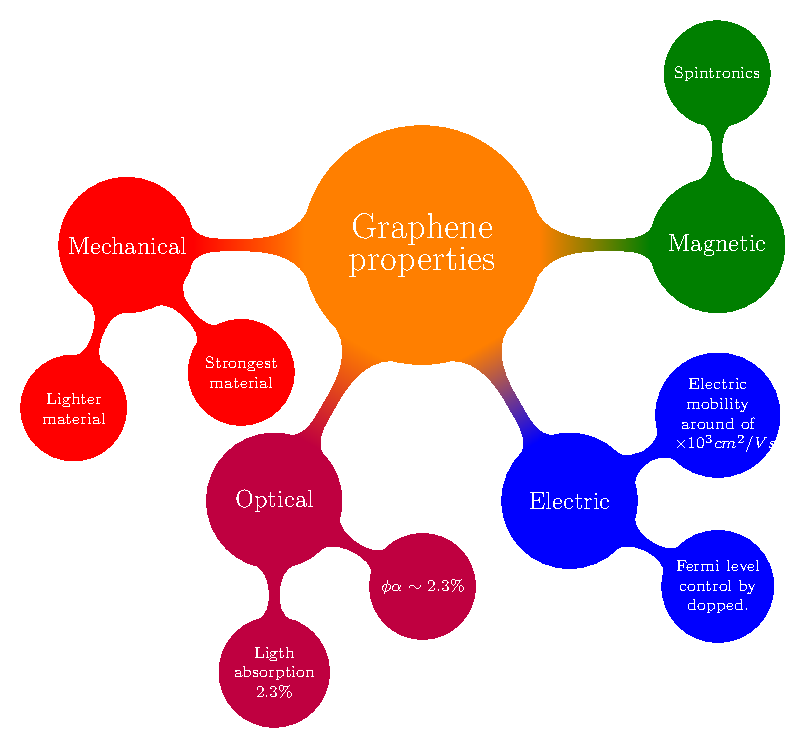
\includegraphics[width=\textwidth]{FIGURES/Physical_Background/image07.pdf}
	\caption{Applications}
	\label{fig:introfig32}
\end{figure}




\section{Graphene structures}
\vspace{-1cm}
Graphene is defined as a novel two-dimensional sheet of atomic thickness which is organized in a hexagonal honeycomb lattice of $sp2$-hybridized carbon atoms (a 2s orbital is mixed with two of the 2p orbitals and a total of 3 hybrid orbitals can form covalent bonds, called $\sigma$ bonds with neighboring carbon atoms).  It has been extensively invesgated since Geim and Novoselov first isolated it by performing mechanical exfoliation based on repeated peeling of highly oriented pyrolyzed graphite. For their pioneering work, which revealed the exceptional physical properties of graphene, Geim and Novoselov were awarded the 2010 Nobel Prize in Physics. 
Graphene has extraordinary thermal, electronic and mechanical properties, which have generated great expectations for various applications like  energy storage , solar cells \cite{singh2015graphene} and conversion, biosensors \cite{yang2015graphene,shao2010graphene}, biocompatible materials \cite{pinto2013graphene}, batteries \cite{kucinskis2013graphene}, optoelectronics, electronics \cite{schwierz2010graphene,chee2016flexible,li2012review} and the latter is still facing challenges\cite{mullen2017polyphenylenes}.  To date it has been extensively researched and a large number of papers have been published showing evidence of its properties and thus applications. 
\begin{figure}
	\centering
	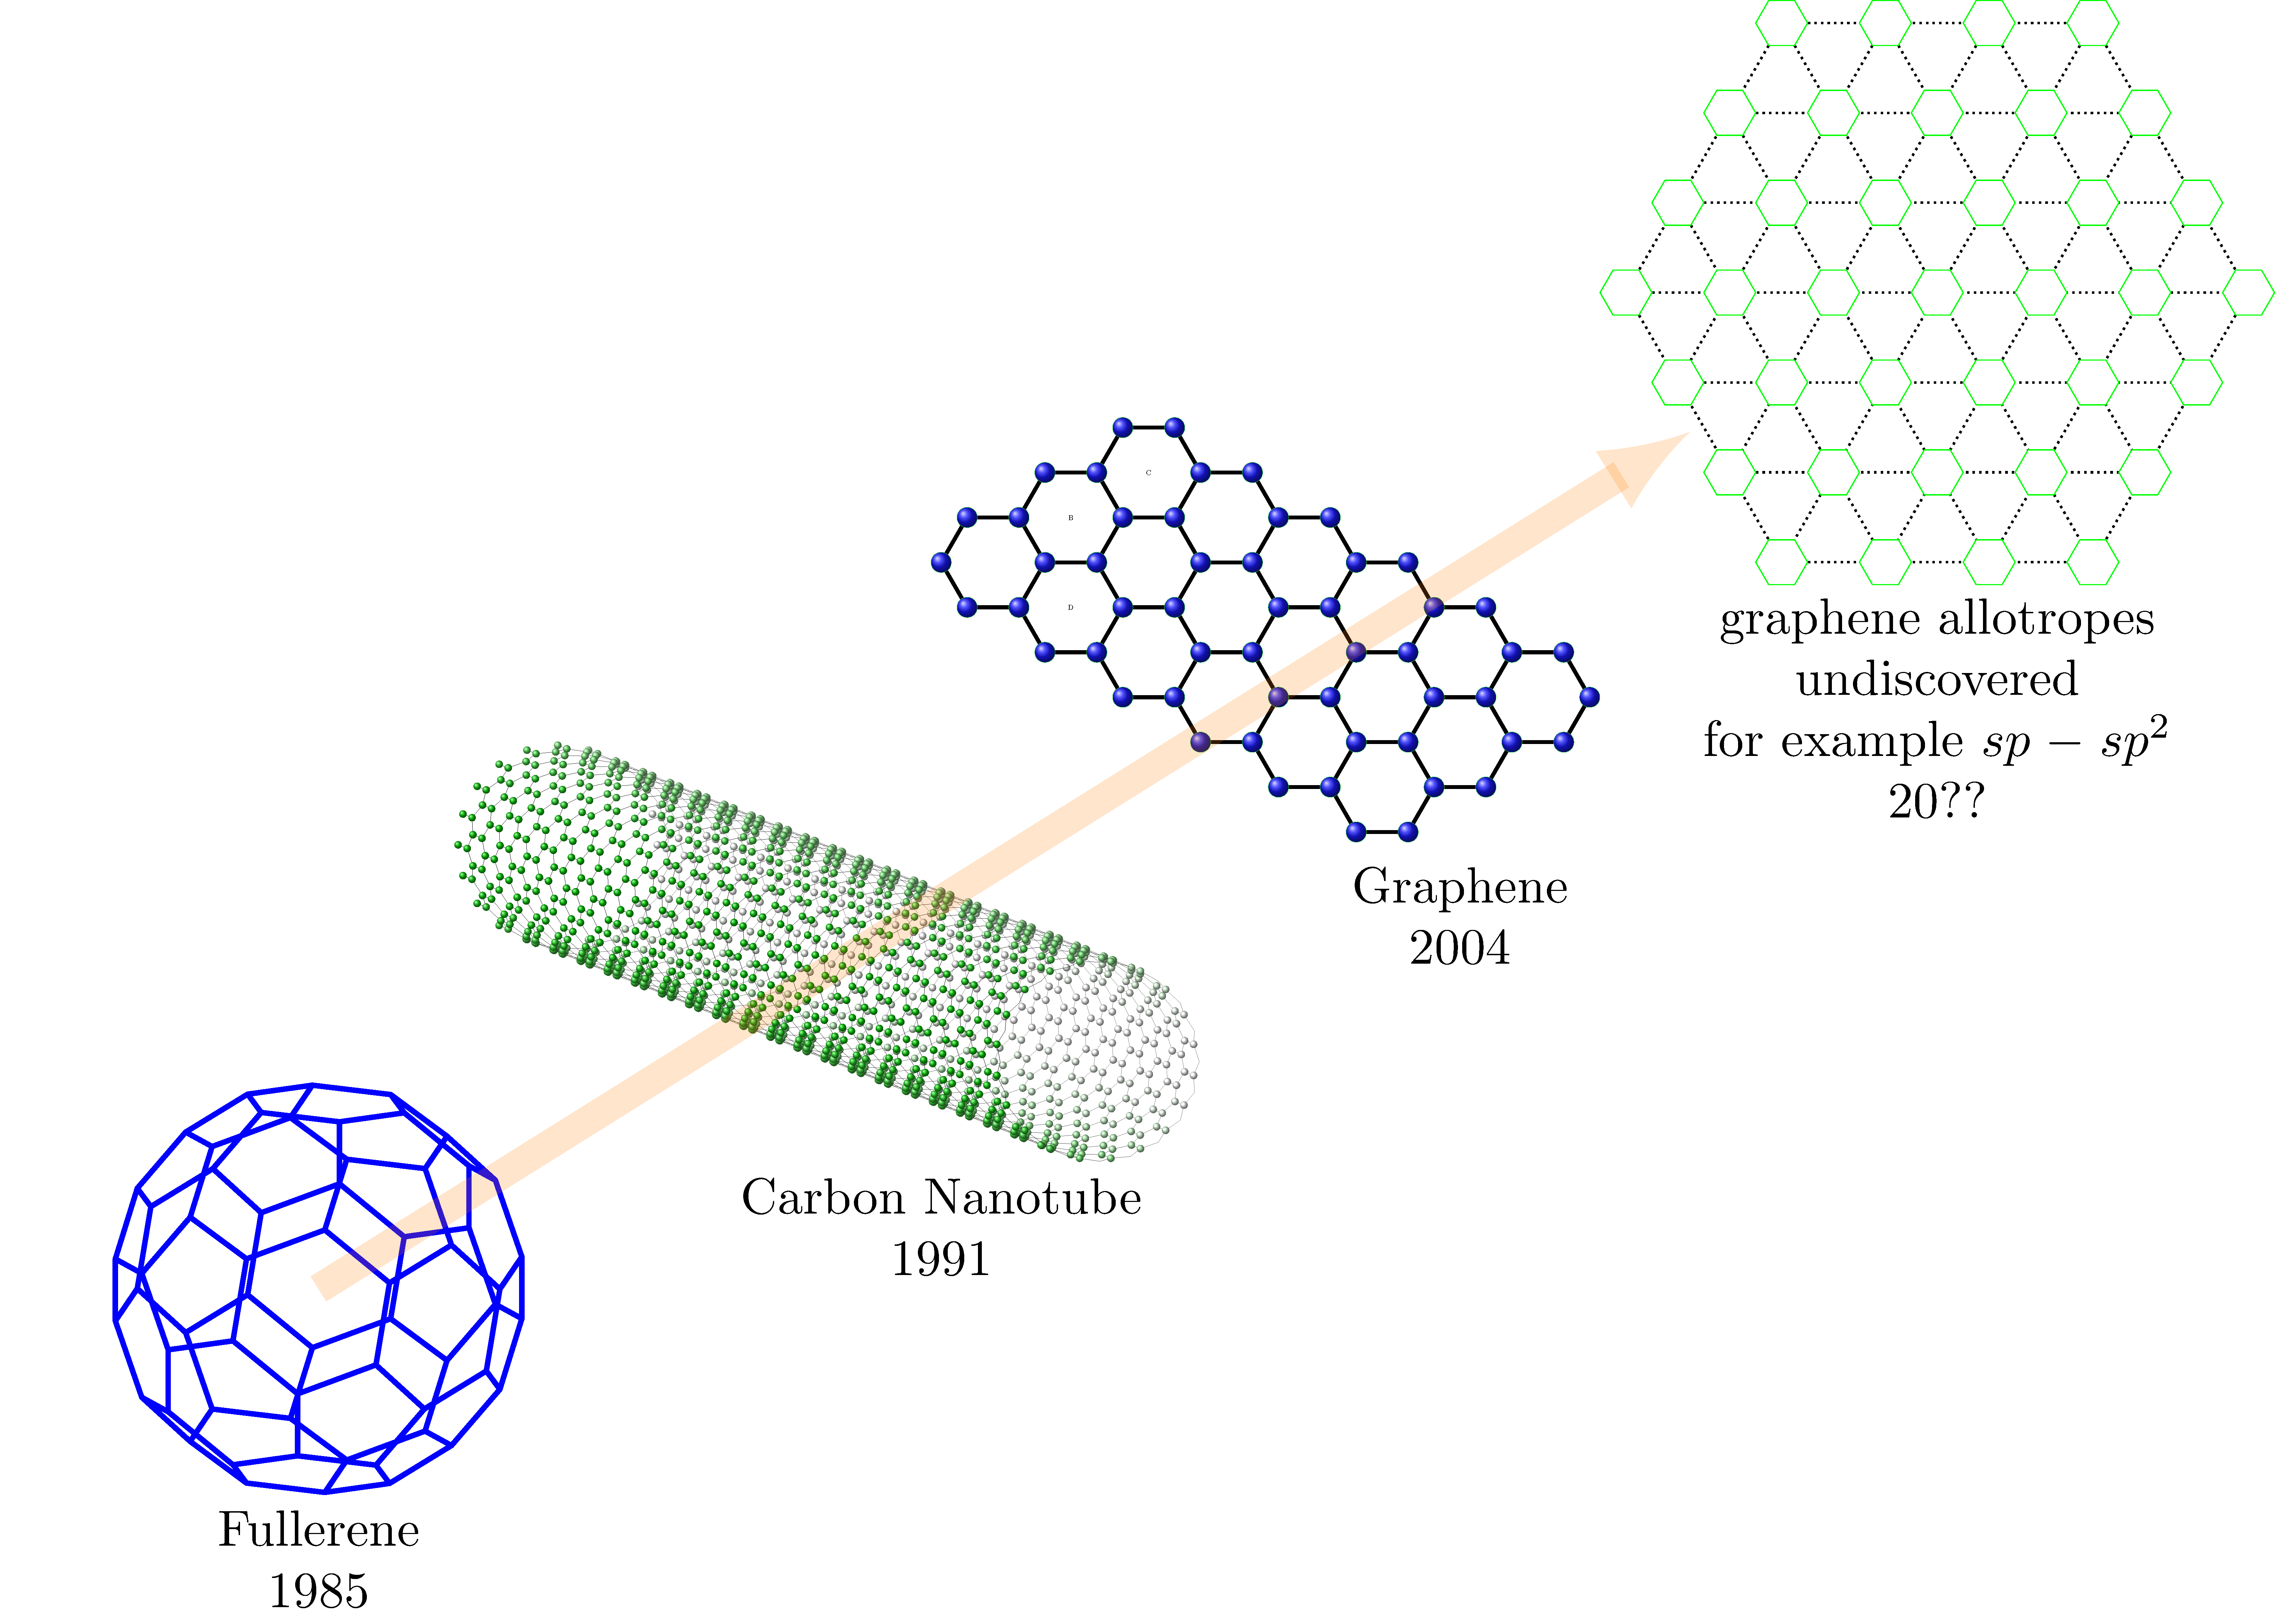
\includegraphics[width=0.8\linewidth]{FIGURES/Introduction/Intro_Fig3/Intro_Fig3}
	\caption{Carbon allotrope timeline}
	\label{fig:introfig32}
\end{figure}
\\
Given the electronic structure of graphene there are some applications that are not possible, a clear example is when you require a device you need to have an off-on process and that is why semiconductors (considerable gap) are optimal for these technological applications, however graphene has no gap and this makes it impossible to stop the flow of current so it is practically impossible to turn off at any reasonable temperature because in graphene large populations of carriers are easily produced by thermal energy and fluctuations. It is then that arises the search to induce a band gap with these graphene structures has been done much research in this area and we can mention some ways to open the gap in these structures i) applying uniaxial strain \cite{ni2008uniaxial}  ii) by dopants however this modifies the properties of graphene itself as it is a modification in the mobility of the same, iii)Graphene can grow epitaxially on SiC to form ribbons (GNRs) with widths controlled by growth conditions and post-growth annealing procedures \cite{celis2016graphene,baringhaus2014exceptional,sprinkle2010scalable}. The band gap of GNRs is a function of the ribbon width and that is why controlled growth followed by reliable determination of properties such as width and thickness is of fundamental importance to tailor the properties of these nanostructures to specific applications\cite{flores2021optical}.


\begin{figure}[H]
	\centering
	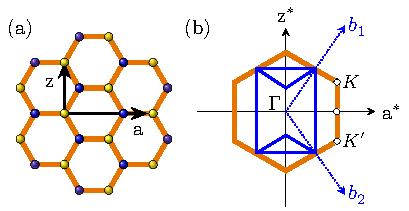
\includegraphics[width=0.82\linewidth]{FIGURES/Physical_Background/Teoria_Fig5.pdf}
	\caption{uno-dos}
	\label{fig:sq-how to reflex}
\end{figure}


\begin{figure}[H]
	\centering
	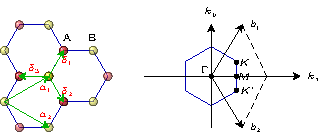
\includegraphics[width=0.85\linewidth]{FIGURES/Physical_Background/Teo_fig1.pdf}
	\caption{uno-dos}
	\label{fig:sq-how to reflex}
\end{figure}

The structure can be seen as a triangular lattice with a base of two atoms per unit cell. The vectors are described as follows: 

\begin{equation}
	a_{1}=\frac{a}{2}(3, \sqrt{3}), 
	a_{2}=\frac{a}{2}(3, -\sqrt{3}),
\end{equation}
 Donde $a\approx 1.42\AA$ y sus vectores de la red reciproca estan dados por 
 \begin{equation}
	b_{1}=\frac{2 \pi}{3a}(1, \sqrt{3}), b_{2}=\frac{2 \pi}{3a}(1,-\sqrt{3})
 \end{equation}

\begin{figure}[h!]
	\centering
	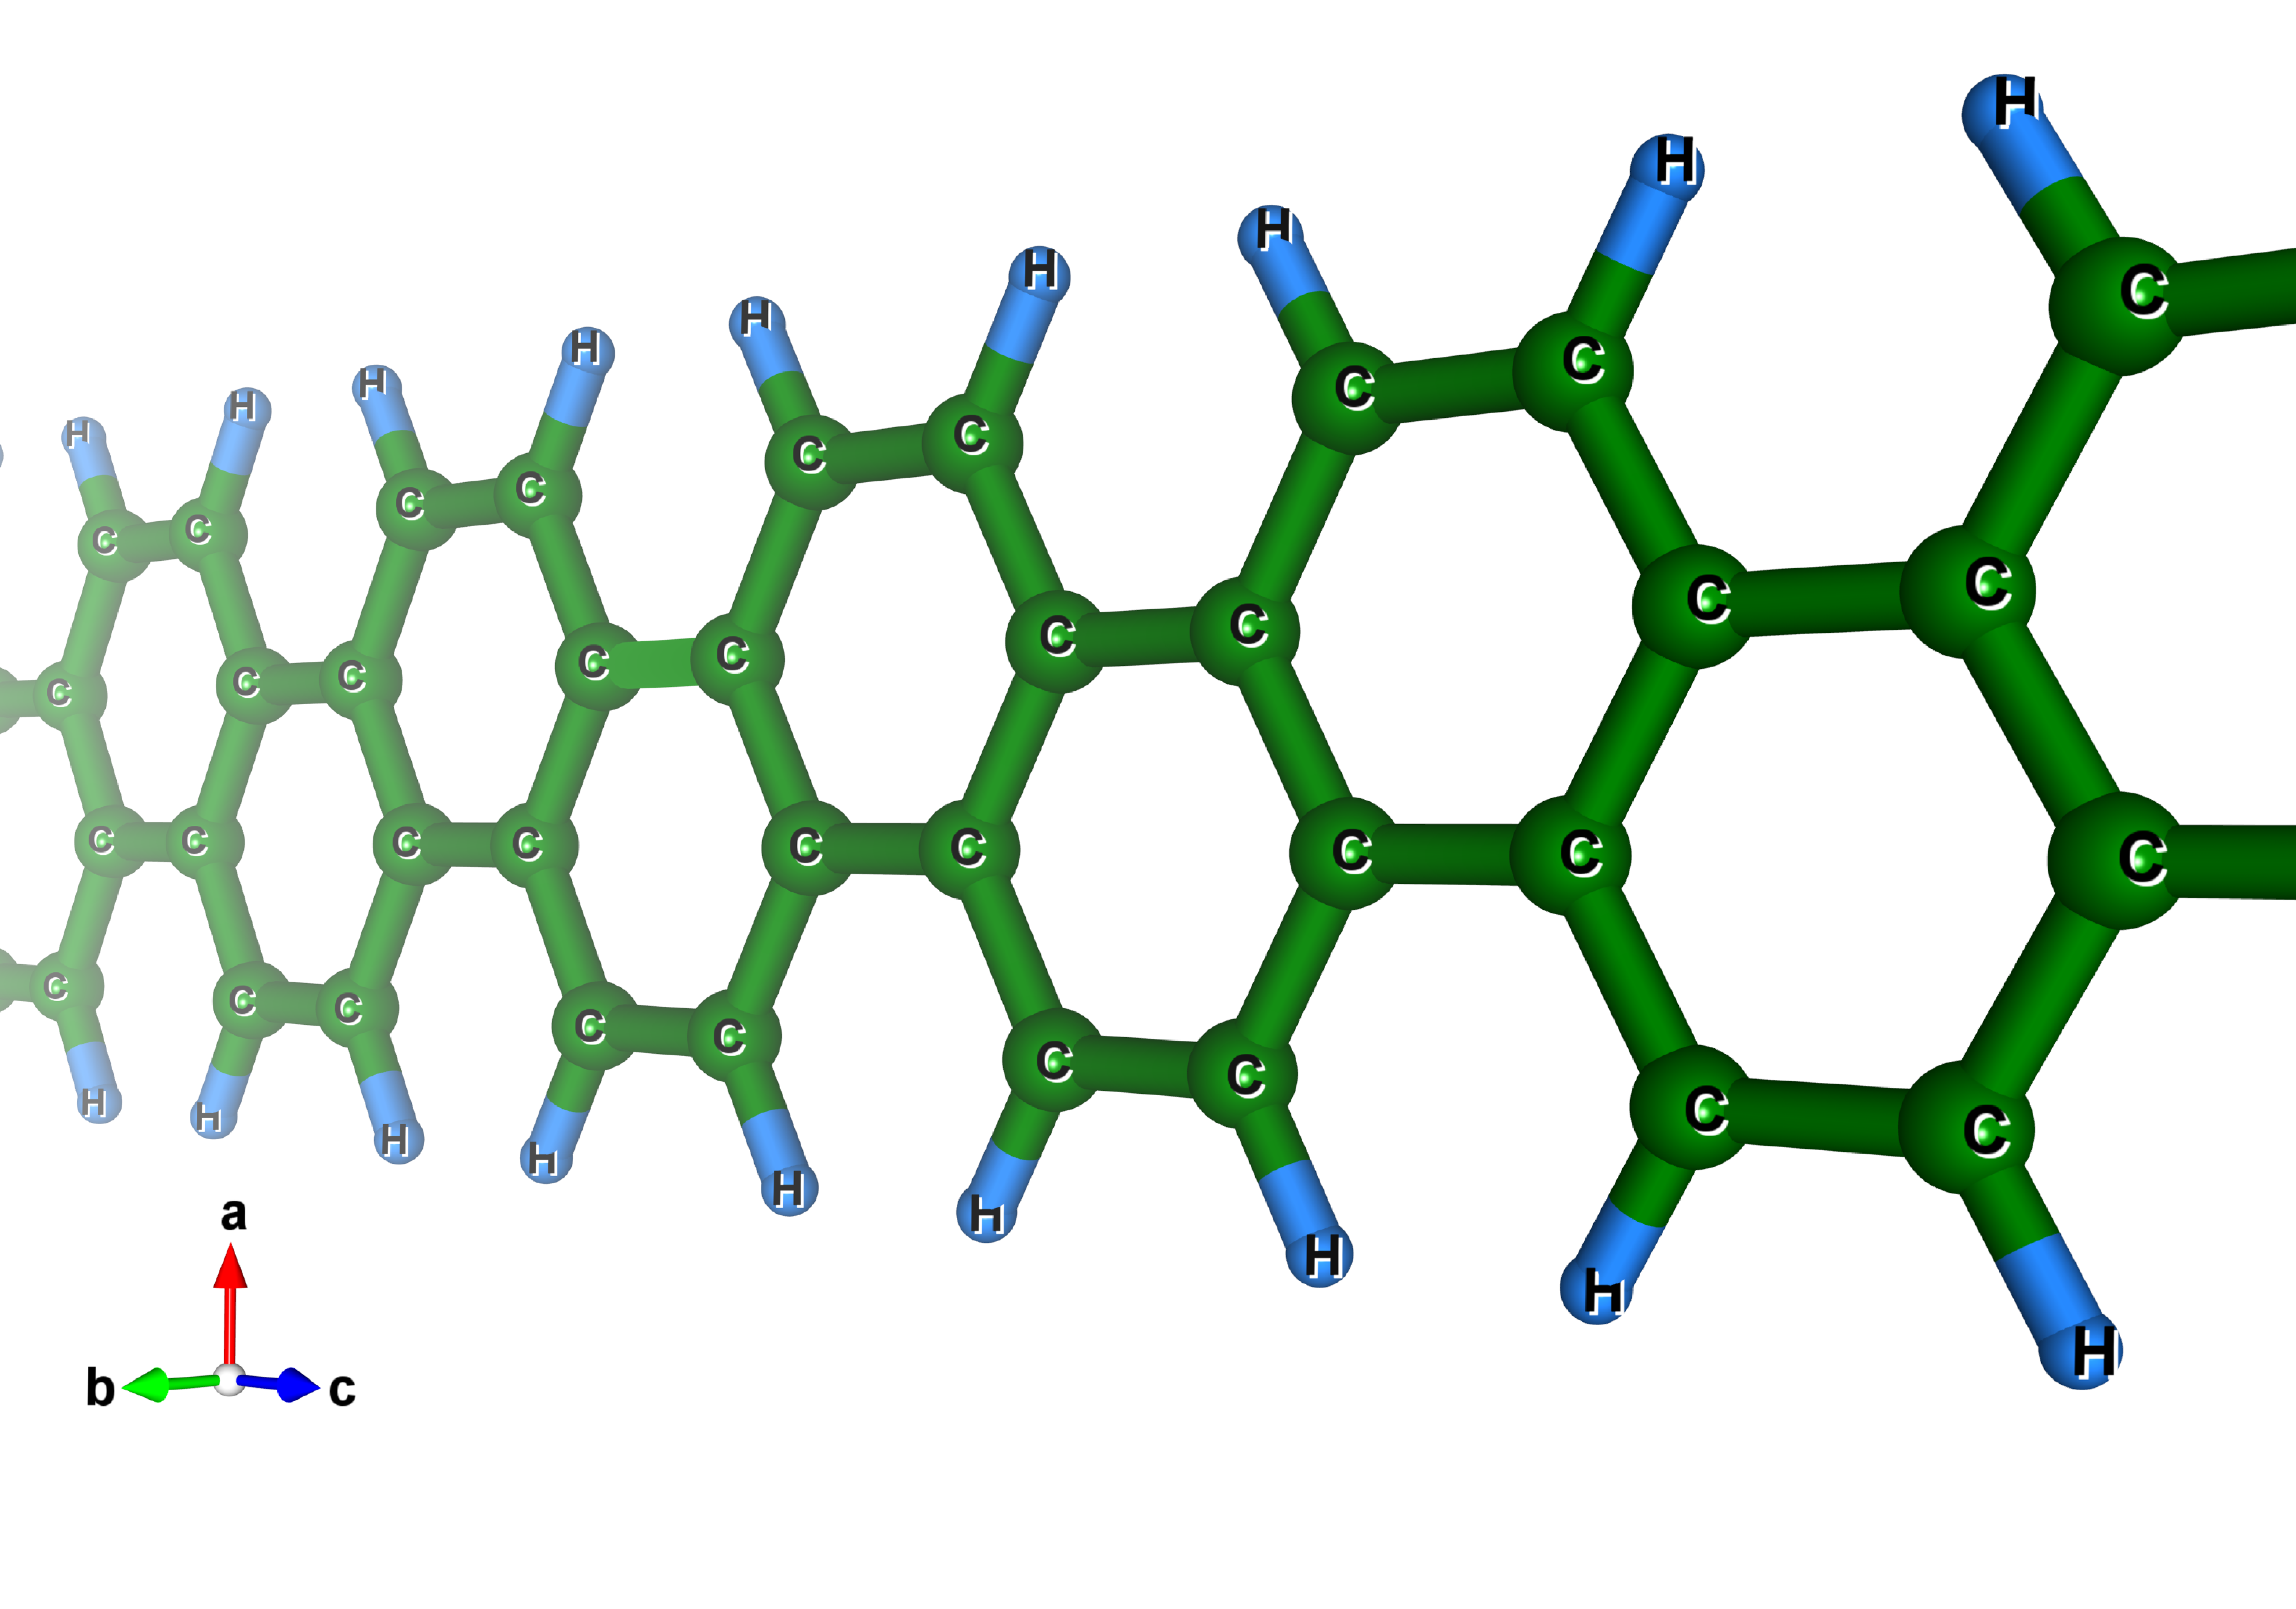
\includegraphics[width=0.80\linewidth]{FIGURES/Physical_Background/GNR-1}
	\caption{Structure of armchair GNRs, which are the ones we study throughout this thesis, are schematized with H at the end bonds. }
	\label{fig:introfig32}
\end{figure}


\subsection{Graphene Monolayers and Bilayers}
\vspace{-1cm}
The atomic structure of carbon allows it to be used in different configurations such as i) folded into fullerenes (0D), ii) rolled into nanotubes (1D), iii) stacked into graphite (3D). The carbon atoms of graphene are separated by an interatomic distance of $a=1.42\angstrom$ and the primitive cell of graphene is composed of two non-equivalent atoms. As for its electronic configuration it is very important to mention that the planar orbitals form the energetically stable and localized $\sigma$ bonds with the three nearest carbon atoms in the honeycomb lattice, and are responsible for most of the binding energy and elastic properties of the graphene layer so that the remaining 2pz orbitals have $\pi$ symmetry and the overlap of these orbital states between neighboring atoms plays an important role in the electronic properties of graphene.

\begin{figure}[H]
	\centering
	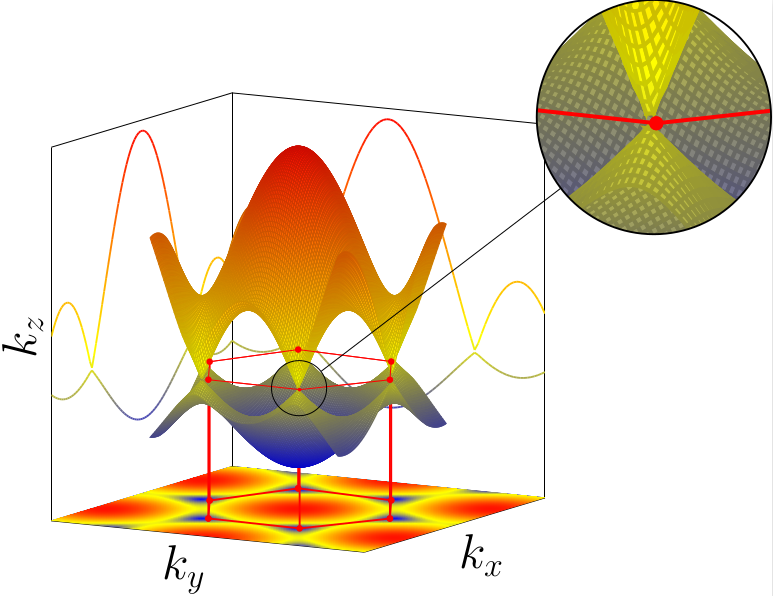
\includegraphics[width=0.75\linewidth]{FIGURES/Physical_Background/bands-graphene.png}
	\caption{a) Band structure of graphene with the respective projections in the $k_y$ and $k_x$ plane, the insight shows the linear dispersion is observed, i.e. near the point $K$ and $K\prime$ (Dirac Point), b)Honeycomb lattice of graphene, showing the unit cell corresponding to two non-equivalent atoms A and B.
	}
	\label[figure]{}
\end{figure}

\subsection{Graphene Nanoribbons}
\vspace{-1cm}
In the case of GNRs it is worth mentioning that many of their essential properties have been conducted by the tight-binding model\cite{nakada1996edge,sohmen1992electronic}and the first-principles method\cite{son2006half}. In the former model GNRs in armchair configuration are predicted to be metals and in the latter they are semiconductors for $N_A=3I+2$ where $N_A$ is the number of dimer lines along the transverse direction corresponding to the electronic states of monolayer graphene in the presence of open boundary conditions. The energy gaps are predicted to be inversely proportional to the width of the nano-ribbons, clearly indicating the quantum confinement effect. In addition, the electronic properties are sensitive to the change in the structure of the edges recalling that there are two configurations i)armchair which are the already described in this work and ii) and zigzag\cite{lin2018structure}
\begin{figure}[H]
	\centering
	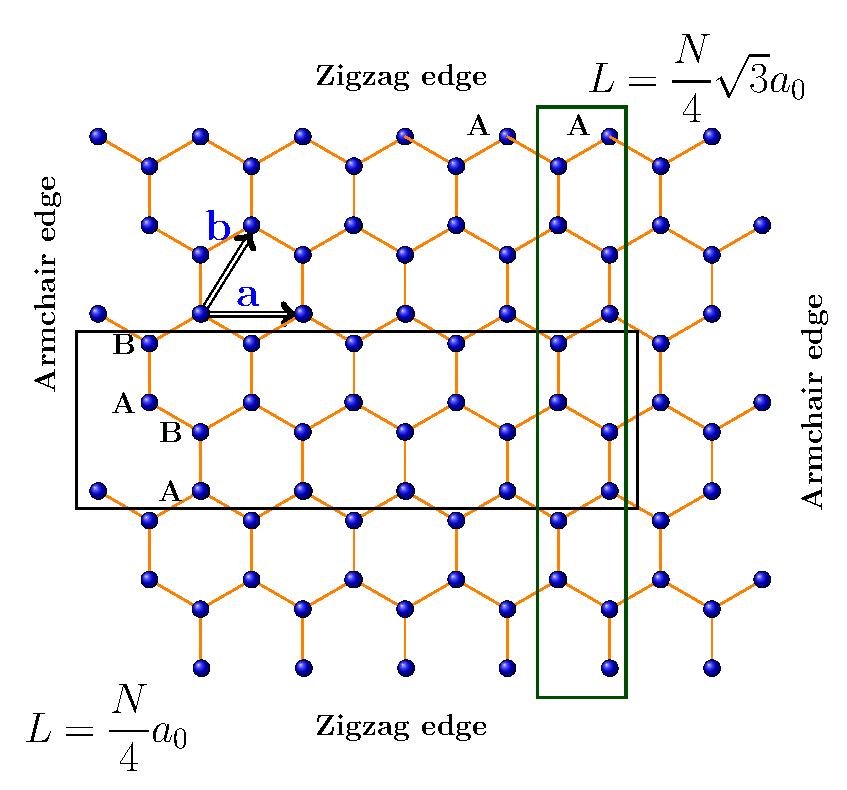
\includegraphics[width=0.75\linewidth]{FIGURES/Physical_Background/Graphene_States.pdf}
	\caption{uno-dos}
	\label{fig:sq-how to reflex}
\end{figure}


\section{Relevant properties}


\subsection{Electronic properties}
\vspace{-1cm}
Graphene is being called as a material of century, although recently two-dimensional materials are the trendy, therefore the interest of graphene was decreased. But, Jarillo-Herrero \textit{et al.}\cite{cao2018unconventional,cao2018correlated,campos2009anisotropic}, they came to get a new hope to Graphene, this due exhibits an  unconventional superconductivity under specific structure arrangement. This behavior and others important them, are exhibits by Graphene and the all gamut of structures derivative of it. Inside that gamut of Graphene structures, the GNR's are very studied by the amazing confinement that these it presents and the interesting applies as spintronic devices\cite{son2006half,kim2007recent}. On going on the physical background involved on it, the geometry of these structures plays the most significant role, due to the \gls{BS} specifically the band gap depends on geometry of these. This means, the ribbon's dimensions affect the band gap value, therefore the properties that can being exhibits depends on that\cite{son2006energy}. In order to illustrate, we worked on first-principle calculations trough preset models without intention of deepens and discuss them, since this work has the aim of show experimental results obtained in this and another structures. But, it is important to break the paradigm that the experimental physicist  does not  can implement masterly tools created by the theorist.  


\subsubsection{Fist approximation of numerical results}
\vspace{-1cm}
The importance of employed theoretical and numerical models to improve and enhanced the understanding of results in solid and condensed matter physics was evolved by technics as Density Functional Theory. As an increasing computational  capacity, it is enabled to employ more sophisticated numerical approximations taken  DFT as basis. This impact in the experimental area, because provides a guide to carried out experiments and structure design\cite{zangwill2015density} with  possibility to get new properties. By this reason, in this works we consider this technics already implemented  in powerful  open codes and  by simplicity and usefully environment, we use ASE interface\cite{ask2017ase}. Since ASE provides the most useful open tools in atomistic simulations, being that their python programming supply and reduce the extensive work. It is important to remark that the fundamental theory discussion will not be addressed in here, we focus on the models and technics as experimental tools therefore we discuss the results getting it. Due to the little computational resource, we purpose two \gls{GNRs}  structures computes trough GPAW code\cite{electronic2010enkovaara,real-space2005mortensen}, GPAW is a density-functional theory (DFT) Python code based on the projector-augmented wave (PAW)\cite{rostgaard2006exact,blochlprojector1994}.
\begin{figure}[ht!]
	\centering
	\includegraphics[width=0.50\linewidth]{FIGURES/Physical_Background/dft001.pdf}
	\caption{}
	\label{fig:intro-dft-structure}
\end{figure}
 Taking advantage of ASE environment provides some nanostructures, we take the nanoribbons function, and we adapt in according to our computational resources. \Cref{fig:intro-dft-structure} shown both zigzag and armchair structures consider in our DFT calculations. With the codes employs in our experimental research these the work are becomes friendly, then is easy to get band structure information. The given results are characteristic by these structures, because as well known the edge plays an importantly role of confinement and the consequently properties of GNRs. This approximate results expose the variety of Graphene zoo results, the simplicity of symmetry around of edge modify also properties and characteristics. The importance of calculate the \gls{BS} 
\begin{figure}[ht!]
	\centering
	\includegraphics[width=\textwidth]{FIGURES/Physical_Background/dft002.pdf}
	\caption{Structure of armchair GNRs, which are the ones we study throughout this thesis, are schematized with H at the end bonds. }
	\label{fig:introfig32}
\end{figure}

\begin{figure}[H]
	\centering
	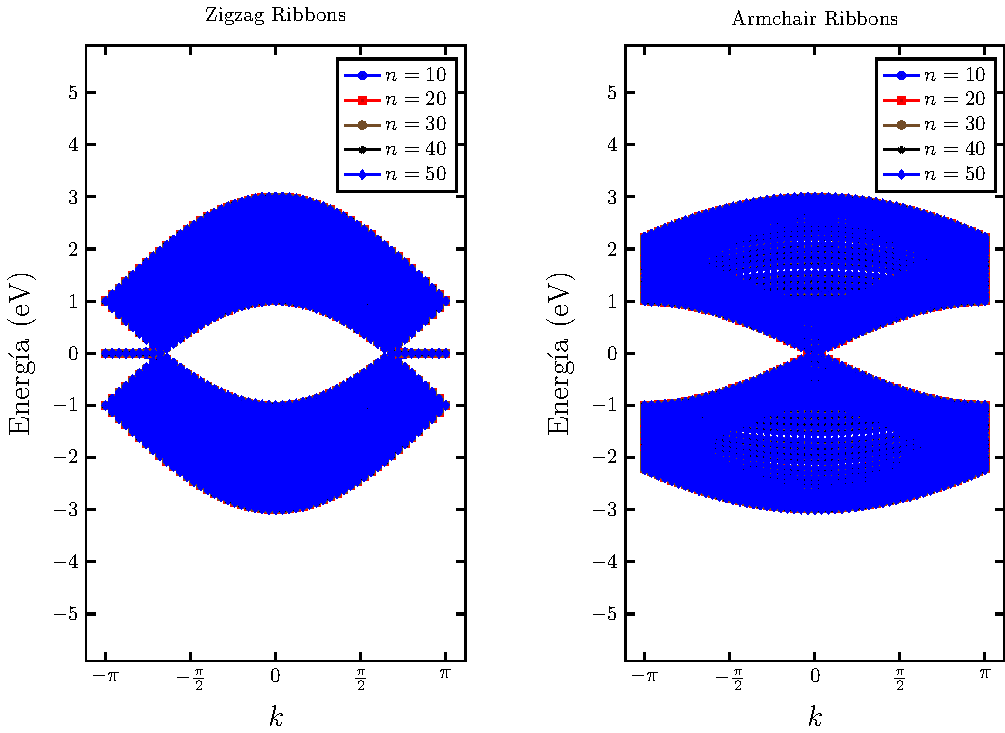
\includegraphics[width=0.82\linewidth]{FIGURES/Physical_Background/Teoria_Fig5b.pdf}
	\caption{uno-dos}
	\label{fig:sq-how to reflex}
\end{figure}

\vspace{-1cm}
The objective in this section of the thesis is to use these existing computational tools to correlate with the experimental results.

\begin{figure}[h!]
	\centering
	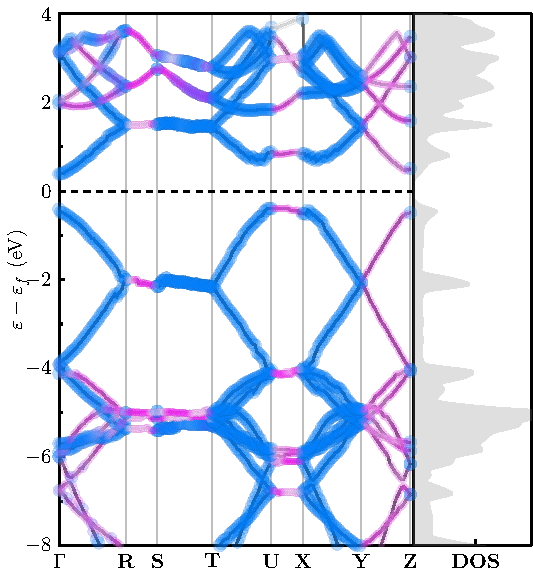
\includegraphics[width=0.80\linewidth]{FIGURES/Physical_Background/PLOT-GNRS007}
	\caption{Structure of armchair GNRs, which are the ones we study throughout this thesis, are schematized with H at the end bonds. }
	\label{fig:introfig32}
\end{figure}


\begin{figure}[h!]
	\centering
	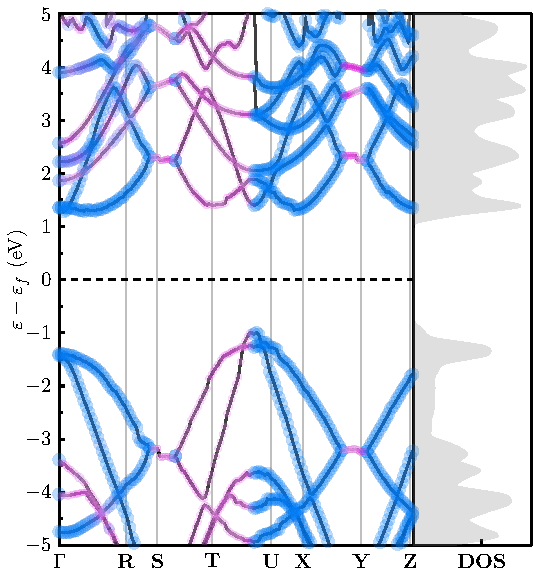
\includegraphics[width=0.80\linewidth]{FIGURES/Physical_Background/PLOT-GNRS008}
	\caption{Structure of armchair GNRs, which are the ones we study throughout this thesis, are schematized with H at the end bonds. }
	\label{fig:introfig32}
\end{figure}
\vspace{-1cm}


The importance of employed theoretical and numerical models to improve and enhanced the understanding of results in solid and condensed matter physics was evolved by technics as Density Functional Theory. As an increasing computational  capacity, it is enabled to employ more sophisticated numerical approximations taken  DFT as basis. This impact in the experimental area, because provides a guide to carried out experiments and structure design\cite{zangwill2015density} with  possibility to get new properties. By this reason, in this works we consider this technics already implemented  in powerful  open codes and  by simplicity and usefully environment, we use ASE interface\cite{ask2017ase}. Since ASE provides the most useful open tools in atomistic simulations, being that their python programming supply and reduce the extensive work. It is important to remark that the fundamental theory discussion will not be addressed in here, we focus on the models and technics as experimental tools therefore we discuss the results getting it. Due to the little computational resource, we purpose two GNRs  structures computes trough GPAW code\cite{electronic2010enkovaara,real-space2005mortensen}, GPAW is a density-functional theory (DFT) Python code based on the projector-augmented wave (PAW)\cite{rostgaard2006exact,blochlprojector1994}.


% \begin{figure}[H]
% 	\centering
% 	\includegraphics[width=0.50\linewidth]{/media/labfiles/ruco/repos/PhD-Thesis/FIGURES/dft/build-ruco/dft001.pdf}
% 	\caption{}
% 	\label{fig:intro-dft-structure}
% \end{figure}

 Taking advantage of ASE environment provides some nanostructures, we take the nanoribbons function, and we adapt in according to our computational resources. \Cref{fig:intro-dft-structure} shown both zigzag and armchair structures consider in our DFT calculations. With the codes employs in our experimental research these the work are becomes friendly, then is easy to get band structure information. The given results are characteristic by these structures, because as well known the edge plays an importantly role of confinement and the consequently properties of GNRs. This approximate results expose the variety of Graphene zoo results, the simplicity of symmetry around of edge modify also properties and characteristics. The importance of calculate the \gls{BS} 

% \begin{figure}[H]
% 	\centering
% 	\includegraphics[width=\textwidth]{/media/labfiles/ruco/repos/PhD-Thesis/FIGURES/dft/build-ruco/dft002.pdf}
% 	\caption{Structure of armchair GNRs, which are the ones we study throughout this thesis, are schematized with H at the end bonds. }
% 	\label{fig:introfig32}



\section{Importance of the optical characterization}
\vspace{-1cm}
In addition to the interest of graphene layers (from 1 layer up to 10), graphene nanostructures such as the ones we have studied which are GNRs show a wide interest for various potential electronic applications. It has been studied that nanostructures can offer a direct band gap due to quantum confinement of charge carriers and that it depends on both lateral width and termination which is required for switching devices and even for DNA sequencing tools. 